\documentclass{article}
\usepackage{graphicx} % Required for inserting images
\usepackage{amsmath}
\usepackage{amssymb}
\usepackage{amsthm}
\usepackage{mathrsfs}
\usepackage{hyperref}
\usepackage{tikz}
\usepackage{enumitem}
\usetikzlibrary{graphs.standard}

% PUT COMMANDS HERE
% ------------------------------
\newcommand{\question}[1]{\item (\textbf{#1})}
\newcommand{\answer}{\item[\textbf{\textit{solution:}}]}
\newcommand{\dif}{\mathop{}\!\mathrm{d}}

\theoremstyle{remark}
\newtheorem*{remark}{Remark}
\newtheorem*{note}{Note}

% ------------------------------

\author{Various Tutors}

\begin{document}

% \title{Math 239 Fall 2023 Tutorial Questions Week 1}

\date{2023 Sep. 14/15}
\maketitle

\begin{enumerate}
    \question{Combinatorial Identity 1} Give a combinatorial proof (that is, by counting the same set in two different ways), of the following identity:
    \begin{align*}
        \sum^n_{k=1}\sum^{k-1}_{j=0}{{k-1}\choose j} =2^n-1.
    \end{align*}
    
    \question{Counting Two Ways} Give a combinatorial argument (that is, by counting the same set in two different ways), of the following identity: 
    \begin{align*}
        7{n \choose 7}=n{n-1\choose 6}.
    \end{align*}

    
    \question{Multisets and Monomials} A \emph{monomial} in the $n$ variables $x_1,x_2,...,x_n$ is an expression of the form 
    \begin{align*}
        x_1^{a_1}x_2^{a_2}...x_n^{a_n}
    \end{align*}
    where each $a_i\in\mathbb{N}$. The \emph{degree} of the monomial $x_1^{a_1}x_2^{a_2}...x_n^{a_n}$ is the sum $\sum^n_{i=1}a_i$.

    Give a bijection between the set of monomials of degree $k$ in the variables $x_1,x_2,...,x_n$ and the set of $k$-element multisets with elements of $n$ types. 
    
    \question{Evens and Odds} For $n\geq 1$, give a bijecctive proof of the following identity:
    \begin{align*}
        \sum_{\text{k is even}} {n \choose k}=\sum_{\text{k is odd}}{n \choose k}.
    \end{align*}

    For a bijective proof, you need to describe two sets $A$ and $B$ whose sizes correspond to the LHS and RHS, write down a function $f: A\rightarrow B$, show that $f(x)\in B$ for all $x\in A$, write down the inverse function $f^{-1}$, and show that $f^{-1}(y)\in A$ for all $y\in B$. In general you need to prove that $f$ and $f^{-1}$ are actually inverses of each other, but you will not have to do that in this problem. 
    
\end{enumerate}
% \title{Math 239 Fall 2023 Tutorial Questions Week 2}

\date{2023 Sep. 21/22}
\maketitle

\begin{enumerate}
    \question{Even and Odd} For any integer $n \geq 0$, determine the number of compositions of $n$ 
    with $3$ parts where exactly $2$ parts are even.  You need to define 
    a relevant set, a weight function, determine a generating series, 
    and find an explicit formula for the answer.  

    
    \question{Power Series} Find the power series generating functions for each of the following sequences in closed form. Each sequence is defined for all $n \ge 0$.
    \begin{itemize}
        %\item $a_n = n^2$
        \item $a_n = 3^n$
        \item $a_n = 3 \cdot 7^n - 5 \cdot 4^n$
    \end{itemize}
    % let me know if this question is reasonable, I feel like the first bullet might not be since it uses derivatives which I haven't seen in the course notes so I commented it out
    % Who is "me"? In any case I think it would be cool to do it in reverse, ie give the generating function that produces $n^2$ and tell them to show it gives $n^2$. I have written this up below. Also I think that doing this way would be a bit much since most often people do not cover derivatives. -- Alex
    % I have talked to instructor and they said that they will not cover derivatives in class and we should not put them on the tutorial at risk of confusion. --Alex
    % I got excited about it and wrote it up as a bonus question anyway, which I'll put as question 5 with a lot of warning symbols around it. I also okayed this with a prof. -- Alex

   
    
    \question{Some Less-Usual Coefficient Extraction} Let $a,k,l$ be constants. Find the following coefficients.
    \begin{enumerate}
        \item $[x^n] \left[ \frac{1}{2-x^2} \right]$.
        \item $[x^n] \left[ \frac{1}{1-x} \cdot \frac{1}{1-3x} \right]$.
        \item $[x^n] \left[ (1+ax)^k \right]$.
        \item $[x^n] \left[ (1+x^l)^k \right]$.
    \end{enumerate}
    For the last one you might need to put on your Math 135 hat!
    \question{Sum Lemma} Let $\mathscr{S} = \{1, 2, 3, 4, 5, 6\}^4$ be the set of outcomes when rolling four six-sided dice. For $(a, b, c, d) \in \mathscr{S}$, define its weight to be
$\omega(a, b, c, d) = a + b + c + d$. Consider the generating series  $\Phi_\mathscr{S}(x)$ of $\mathscr{S}$ with respect to $\omega$.
\begin{enumerate}
    \item Explain why $\Phi_\mathscr{S}(x) = \left(\frac{x-x^7}{1-x}\right)^4$
    \item How many outcomes in $\mathscr{S}$ have weight 19?
    \item Let $m,d,k$ be positive integers. When rolling $m$ dice, each of which has exactly $d$ sides (numbered with $1,2, \dots, d$ pips, respectively), how many different ways are there to roll a total of $k$ pips on the top faces of the dice? (Part (b) is the case $m=4, d=6, k = 19$.)
\end{enumerate}


    % This following question is from Alex
    \question{Bonus Material: Formal Derivatives} This is not $239$ material and will not be covered in $239$. You should not use this notation or train of thought for assignments or tests.
    
    Consider a generating function
    \begin{align*}
        A(x) = \sum_{i=0}^\infty a_i x^i = a_0 + a_1 x + a_2 x^2 + a_3 x^3 + \cdots.
    \end{align*}
    We define the \textit{formal derivative} of $A(x)$ to be
    \begin{align*}
        \frac{\dif}{ \dif x} A(x) = \sum_{i = 1}^\infty i a_i x^{i-1} = 1 a_1 + 2 a_2 x + 3 a_3 x^2 + 4 a_4 x^3 + \cdots.
    \end{align*}
    \begin{enumerate}
        \item Find $[x^n] \left[ \frac{\dif}{\dif x} A(x) \right]$.
        \item Find $[x^n] \left[ x \frac{\dif }{\dif x} A(x)  \right]$.
        \item Using the \textit{formal derivative} as a ``normal derivative", ie treating the derivative like you would in a first calculus course, find the generating function for the following sequences.
        \begin{enumerate}
            \item $a_n = n$.
            \item $a_n = n^2$.
            \item $a_n = n^k$ for any fixed $k \geq 1$.
        \end{enumerate}
    \end{enumerate}
    \begin{remark}
        The last one might be hard/impossible, but it turns out if you care only about the \textit{asymptotic behaviour} of $a_n$, that is you want $a_n$ to be approximately $n^k$ for large enough $n$, it is much easier. A result from \textit{analytic combinatorics} says that one example of a generating function for a sequence like this is $\frac{k!}{(1-x)^{k+1}}$ (in fact by the math software Sagemath, then $[x^{1000}] \frac{4!}{(1-x)^5} \approx 1.01004513028955 \cdot (1000)^4$, which shows that at $n=1000$ there is only about a $1 \%$ error).
    \end{remark}
\end{enumerate}
% \title{Math 239 Fall 2023 Tutorial Questions Week 3}

\date{2023 Sep. 28/29}
\maketitle

\begin{enumerate}
    \question{Ambiguous Expressions} Let $S$ be the set of all strings where each block has even length.
    \begin{enumerate}
        \item Come up with an unambiguous expression for $S$. Justify in about a sentence why this is unambiguous.
        \item Using your unambiguous expression, find the generating function for $S$ (with respect to length). What do you notice?
        \item Using your unambiguous expression, find the generating function for $S$ with the weight function $w(0) = 1$ and $w(1) = 2$.
        \item Come up with an \textit{ambiguous} expression for $S$ and try to find the generating function for $S$ (with respect to length) using it. Compare the coefficients with your coefficients from (b). What do you notice? What will you notice in general?
    \end{enumerate}
    
    \question{Unambiguous Expressions} 
    \begin{enumerate}
        \item Provide an unambiguous regular expression ${\rm R}$ that produces the set of all binary strings that begin and end with the same bit (this includes the empty string).  What rational function does ${\rm R}$ lead to? 
        \item Let $\mathcal{S}$ be the set of all strings where any occurrence of 1 must be immediately followed by at least 5 consecutive 0’s.  Find an unambiguous regular expression ${\rm R}$ that produces $\mathcal{S}$, and provide the rational function that ${\rm R}$ leads to.     \end{enumerate}
    
    \question{Compositions} Let $\mathcal{E}$ be the set of compositions $\gamma= (c_1, c_2, \cdots, c_k)$ of any length, in which part $c_i$ is congruent to $i$ (modulo $2$). We consider empty composition $\epsilon = ()$ in the set $\mathcal{E}$. 

    Express the set in terms of disjoint unions/Cartesian products, then obtain the generating series of the set with respect to size as a rational function.
    
    \question{Generating Series} Determine the generating series, with respect to length, for the number of binary strings of length $n$ which start with a 0, end with a 1, and do not contain 0 as a block. Write out the first four non-zero terms of the generating series and the corresponding strings.


    \question{Bonus Material: A Second GF for Binomial Coefficients} This is not $239$ material and will not be covered in $239$. You should not use this notation or train of thought for assignments or tests. This is intended as a challenging question for people who are interested.
    
    Single-variate generating functions are familiar to us at this point in the course. We can similarly define bi-variate generating functions as formal power series
    \begin{align*}
        A(x,y) =  \sum_{i \geq 0} \sum_{j \geq 0} a_{i,j} x^i y^j.
    \end{align*}

    A familiar GF to us is the GF for binomial coefficients with respect to ``$k$"
    \begin{align*}
        \sum_{k \geq 0} \binom{n}{k} x^k = (1+x)^n.
    \end{align*}
    Using this, and the notion of a bi-variate generating function, find a closed form for the GF for binomial coefficients with respect to ``$n$"
    \begin{align*}
        \sum_{n \geq 0} \binom{n}{k} y^n.
    \end{align*}
    
\end{enumerate}
% \title{Math 239 Fall 2023 Tutorial Questions Week 4}

\date{2023 Oct. 05/06}
\maketitle

\begin{enumerate}
    \question{Warm-up Recursive Expressions}
    \begin{enumerate}
        \item Write both a regular expression and a recursive decomposition for the set of binary strings, where each block of $1$'s has even length. Find the generating function for both of these expressions and ensure that they are the same.
        \item Write a recursive expression for the set of strings of length $n$ such that if there is a $1$ at position $j $ there is a $0$ at position $n+1-j$ and if there is a $0$ at position $j$ then there is a $1$ at position $n+1-j$.
        
        For example consider a string
        \begin{align*}
            a_1 a_2 a_3 \cdots a_{n-2} a_{n-1} a_n.
        \end{align*}
        Then if $a_2 = 0$ we must have that $a_{n+1-2} = a_{n-1} = 1$. Find the generating function of these.
        Is it possible to write this using a non-recursive expression? If yes give it, if not say why.
    \end{enumerate}
   
    
    \question{Partial Fractions} Use partial fraction decomposition to produce a closed-form formula for the coefficients
    \[q_n = [x^n] \frac{18+12x}{1-9x^2}\]

    \newpage
     
    \question{Avoiding Substrings}
        In this question we will use recursive decomposition to count the number of binary strings with length $n$ that do not contain $011$ as a substring. 
        \begin{enumerate}
             \item Let $S$ be the set of binary strings avoiding 011 as a substring, and let $T$ be the set of binary strings containing exactly one occurrence of 011 at the very end. Find two equations of sets $S$ and $T$. Justify your equations. 
             \item Deduce the generating series for $S$ with respect to the length of the strings.
             \item (Partial Fraction Challenge Part) Express the number of binary strings with length $n$ that do not contain $011$ as a substring as a function of $n$ in closed form.
        \end{enumerate}

        
    \question{Recurrence}  Let ${a_n}$ be the sequence which satisfies
    
        \begin{center}
            $a_n - 2a_{n-1} - 7a_{n-2} - 4a_{n-3} = 0$
        \end{center}

        for $n \ge 3$ with initial conditions $a_0 = 3$, $a_1 = 7$, $a_2 = 8$. Determine an explicit formula for $a_n$. 


    \question{Counting Binary Trees and Dyck Paths}

    Define a full binary tree to be a binary tree where each vertex has either $0$ or $2$ children. Often we can realize trees and other combinatorial structures recursively. Probably the most popular example is realizing that a full binary tree is either empty, or a vertex followed by two full binary trees.
    \begin{enumerate}
        \item Justify that this gives us the GF relationship
        \begin{align*}
            B(x) = 1 + x \cdot B(x) \cdot B(x) = 1 + xB(x)^2.
        \end{align*}
        Solve this for $B(x)$ and justify which of the two solutions is the legitimate one.
        \item Using the generalization of binomial expansion in \url{https://en.wikipedia.org/wiki/Binomial_series}, find a closed-form expression for the number of binary trees with $n$ vertices (ie find $[x^n]B(x) =: C_n$).
    \end{enumerate}
    After a lot of algebra this is very amazingly the Catalan numbers! These numbers pop up in the wild quite a lot.
    
\end{enumerate}
% \title{Math 239 Fall 2023 Tutorial Questions Week 5}

\date{2023 Oct. 19/20}
\maketitle

\begin{enumerate}
    \question{A Routine Recurrence} Consider the recurrence
    \begin{align*}
        a_{n+3} + 5 a_{n+2} + 3a_{n+1} - 9a_n = 0
    \end{align*}
    where $a_0 = 1, a_1 = 3, a_2 = 5$. Find an explicit formula for $a_n$. What is our formula for $a_n$ if we set $a_0 =3, a_1 = 9, a_2 = 15$ (ie triple what they were before) instead?
    \begin{note}
        You can use Wolfram Alpha to factor polynomials if you want.
    \end{note}
    
    \question{Another Recurrence} 
    Let \[A(x) = \frac{1}{1-3x-2x^3}\] 
    and let 
    \[a_n = [x^n]A(x).\]
    \begin{enumerate}
        \item What homogeneous linear recurrence is satisfied by the coefficients $a_n$?
        \item What are the initial conditions of this homogeneous linear recurrence?
        \item Invent a set of combinatorial objects such that the number of objects of size n is $a_n$.
    \end{enumerate}
    \question{Degree Sequences} Suppose that $d_1, d_2, \dots, d_n$ are the degrees of a graph $G$, ordered so that $d_1 \ge d_2 \ge \dots \ge d_n$. Then $d_1, d_2, \dots, d_n$ is called the \textbf{degree sequence} of $G$. For each of the following degree sequences, either draw a graph with the degree sequence, or explain why it can't exist.
    \begin{enumerate}
        \item $4, 3, 2, 2, 1$
        \item $6, 5, 4, 3, 2, 1$
        \item $5, 4, 4, 3, 2, 1$
        \item $3, 3, 3, 3, 3, 3$
        \item $2, 2, \dots, 2$ for arbitrary length $n$
        \item $6, 6, 4, 2, 2, 2, 1, 1$
    \end{enumerate}


    
    \newpage
    \question{Graph Complements} Recall that if $G$ is a graph $\overline{G}$, the complement of $G$, has $V(G)=V(\overline{G})$ and $E(\overline{G}=\{uv| uv\notin E(G), u,v\in V(\overline{G})\}$.
    \begin{enumerate}
        \item Let $K_n$ be the complete graph on $n$ vertices. Describe $\overline{K_n}$.
        \item For any $v\in G$ what is $deg_G(v)+deg_{\overline{G}}(v)$?
        \item Find a graph $G$ such that $G\cong\overline{G}$. 
        \item Prove that if $|V(G)|\geq 6$ then either $G$ or $\overline{G}$ contains a triangle.
    \end{enumerate}

     %\newpage
    
    \question{Bonus Question: Fibonacci Recurrences}
    Consider the Fibonacci recurrence given by $f_{n+2} = f_{n+1} + f_n$, where $f_0 = 0$ and $f_1 = 1$. As we know from class and partial fraction decomposition, this has the closed form
    \begin{align*}
        f_n = \frac{(1+\sqrt{5})^n}{2^n \sqrt{5}} -  \frac{(1-\sqrt{5})^n}{2^n \sqrt{5}}.
    \end{align*}
    Notice that the second term goes to $0$ as $n \to \infty$.
    \begin{enumerate}
        \item Find a general formula for the Fibonacci-like recurrence given by $f_{n+2} = f_{n+1} + f_n$, where $f_0 = a$ and $f_1 = b$, where $a,b \in \mathbb{R}$. Then the set of initial conditions is $\mathbb{R}^2$. Conclude that there is a one-dimensional subspace of $\mathbb{R}^2$ such that $f_n \to 0$ when the initial conditions are in this subspace (ie there is a line of possible initial values that make $f_n$ tend to $0$). Compute the line orthogonal to this one. What happens to our sequence when our initial conditions are in this orthogonal line?
        \item (hard) Find a closed form for the Tribonacci numbers, defined by $f_{n+3} = f_{n+2} + f_{n+1} + f_n$, where $f_0 = a_0 , f_1 = a_1 , f_2 = a_2$. Then the set of initial conditions is $\mathbb{R}^3$. This has a (possibly trivial) subspace of initial conditions that make $f_n \to 0$. What is the dimension of it?
    \end{enumerate}
\end{enumerate}
% \title{Math 239 Fall 2023 Tutorial Questions Week 6}

\date{2023 Oct. 26/27}
\maketitle

\begin{enumerate}
    \question{Matching Vertices} Prove that any graph with at least two vertices has two vertices of the same degree.
    \begin{note}
        It may be useful to consider the degree sequence of the graph. 
    \end{note}
    
    \question{Paths and Cycles} Let $G$ be a graph and $k\geq 2$ be the minimum degree of $G$ (denoted $\delta(G)$.
    \begin{itemize}
        \item Prove $G$ has a path of length at least $k$.
        \item Prove $G$ has a cycle of length at least $k+1$. 
    \end{itemize}
    

    
  
    
    \question{Vertices and Edges} Let $G$ be a graph with $n$ vertices and $m$ edges, where $m > \frac{(n-1)(n-2)}{2}$. Show that $G$ does not have a vertex of degree $0$

    \newpage
    
  \question{Bipartite Graph and Walks} For each even $n\geq 2$, let $G_n$ be the graph with vertex set
    $$V(G_n) = \{\sigma \in \{0,1\}^n: \sum_{i=1}^n \sigma_i = n/2\}$$
    and such that there is an edge between vertices $x,y \in V(G)$ if and only if $y$ is obtained from $x$ by replacing a substring $10$ with $01$ or vice versa. For example, $\{1100, 1010\}$ and $\{1010, 1001\}$ are some edges in $G_4$.
    \begin{enumerate}
        \item Prove $G_n$ is bipartite.
        \item Show that there exists a walk between any two vertices in $G_n$, and thus prove that $G_n$ is connected.
    \end{enumerate}

    \question{Moore Graphs}
    We often try to import the language for geometric shapes over to graphs. In this light we define the \textbf{distance} between two vertices as
    \begin{align*}
        \operatorname{dist} (u,v) = \min_{\gamma \in path(u,v)} \operatorname{length}(\gamma)
    \end{align*}
    where $path(u,v)$ is the set of all paths from $u$ to $v$, and the length of a path is the number of edges you cross in the path. We define the \textbf{diameter} of a graph to be
    \begin{align*}
        diam(G) = \max_{u,v \in G} \operatorname{dist} (u,v).
    \end{align*}
    This is a measure of how ``spread out" our graph is; if our graph has lots of edges you expect the diameter to be high, and if the graph has few edges you expect a low diameter.
    
    Let $G$ be $d$-regular and have diameter $k$. Show that
    \begin{align*}
        |V(G)| \leq 1 + d \sum_{i=1}^{k} (d-1)^{i-1}.
    \end{align*}
    A graph in which we achieve equality is known as a \textbf{Moore graph}. Some examples of Moore graphs are odd cycles, complete graphs, and the Petersen graph.
\end{enumerate}
% \title{Math 239 Fall 2023 Tutorial Review Session}

\date{2023 Nov. 02/03}
\maketitle

% \textbf{Please read:} This week the proposed format is have a bunch of rote questions, and just stand at the board and solve them to try to get through as many questions as possible. For this reason a separate sheet with solutions on it is not important to have -- we should have one sheet with both questions and answers. Recall we should each write about 2 questions each. I think it would be better if we aimed for simpler and shorter questions to be able to show people stuff that they may have forgotten or not understood, such as weight functions or how to get a GF from a recurrence. The only thing I think should be long or ``unusual" are proofs, such as bijections and some graph theory proofs.

% Penny should send us the exam soon, which will help quite a bit on designing questions. I suggest that we design questions in approximately the same ratio as the exam (I will write this later here), but not to cover exactly what is on the exam. I suggest that you do not tell anyone that you have seen the exam either.

% Penny has now sent the exam. There are $8$ multiple choice questions and $6$ long-form questions (with multiple parts for each) The question breakdowns are approximately:
% \begin{itemize}
%     \item Basic counting -- $3$ MC
%     \item Coefficient extraction, recursions, and partial fractions -- $1$ MC and $2$ LF
%     \item Generating function and weight functions -- $3$ MC
%     \item Graph theory -- $1$ MC and $2$ LF
%     \item Bijections -- $1$ LF
%     \item Binary strings -- $1$ LF
% \end{itemize}

% \newpage

\begin{enumerate}
    \question{Bijection Question} Let $n \geq k \geq 2$. Let
    \begin{align*}
        U = \{ \text{$k$-element subsets of $\{ 1, \cdots, n\}$} \}
    \end{align*}
    and
    \begin{align*}
        V = \{ (a,b,A) \}
    \end{align*}
    where
    \begin{align*}
        a &\in \{ 1 , \cdots, n \},\\
        b &\in \{ 0, \cdots, n-a \},\\
        A &\text{ is a $(k-2)$ element subset of $ \{ 1, \cdots, b-1 \}$ }.
    \end{align*}
    (I.e. $V$ is the set of all triples like this). Find a bijection from $U$ to $V$ and use this to show that
    \begin{align*}
        \sum_{i=1}^n \sum_{j=0}^{n-i} \binom{j-1}{k-2} = \binom{n}{k}.
    \end{align*}
    \answer Consider a subset $S$ in $U$. Denote the minimal/maximal element of $S$ as $S_{min} \in \{ 1 , \cdots, n\}$ and $S_{max} \in \{ S_{min} , \cdots, n \}$. Then
    \begin{align*}
        S \subseteq \{ S_{min} , \cdots , S_{max} \}
    \end{align*}
    with $S_{min} , S_{max} \in S$. Write
    \begin{align*}
        T = S \setminus \{ S_{min} , S_{max} \} \subseteq \{ S_{min} + 1 , \cdots , S_{max} - 1 \}.
    \end{align*}
    $T$ has $k-2$ elements. Now write
    \begin{align*}
        a &= S_{min} \in \{ 1 , \cdots, n \},\\
        b &= S_{max} - S_{min} \in \{0 , \cdots, n - S_{min} \} =  \{0 , \cdots, n - a \},\\
        A &= T - S_{min} \subseteq \{ S_{min} - S_{min} + 1 , \cdots , S_{max} - S_{min} - 1 \} = \{ 1 , \cdots , b - 1 \}.
    \end{align*}
    Where our $T - S_{min}$ is element-wise subtraction. Then $(a,b,A)$ is a valid element of $V$. Note that this is clearly bijective, with the inverse being
    \begin{align*}
        (a , b ,A) \mapsto \{ a\}  \cup (A+a) \cup \{ a+b \}
    \end{align*}
    with the $A+a$ being once again element-wise addition.

    Now note that
    \begin{align*}
        |V| &= \sum_{i=1}^n \sum_{j=0}^{n-i} \binom{j-1}{k-2}
    \end{align*}
    where $ \binom{j-1}{k-2}$ counts number of ways to get $A$, $\sum_{j=0}^{n-i} \binom{j-1}{k-2}$ counts the number of ways to get $b$ and $A$, and $\sum_{i=1}^n \sum_{j=0}^{n-i} \binom{j-1}{k-2}$ counts the ways to count elements of $T$. It follows that
    \begin{align*}
        \sum_{i=1}^n \sum_{j=0}^{n-i} \binom{j-1}{k-2} = |V| = |U| = \binom{n}{k}.
    \end{align*}
    
    \question{Coefficient Extraction} Determine the value of the following coefficients. 
    \begin{enumerate}
        \item $[x^{20}]3x^2(1-5x^3)^{-4}$
        \item $[x^{20}]3x^2(1-5x^3)^{-4}(1+x^4)^{-2}$
    \end{enumerate}
    \answer \begin{enumerate}
        \item Apply negative binomial theorem:
        \begin{align*}
            [x^{20}]3x^2(1-5x^3)^{-4} &= 3[x^{18}](1-5x^3)^{-4} \\
            &= 3[x^{18}]\sum_{n\geq 0}\binom{n+4-1}{4-1}(5x^3)^n \\
            &= 3[x^{18}]\sum_{n\geq 0}\binom{n+3}{3}5^nx^{3n} \\
            &= 3 \binom{6+3}{3}5^6\\
            &= 3 \binom{9}{3} \cdot 5^6
        \end{align*}
        \item 
        \begin{align*}
            [x^{20}]3x^2(1-5x^3)^{-4}(1+x^4)^{-2} &= 3[x^{18}](1-5x^3)^{-4}(1+x^4)^{-2} \\
            &=3[x^{18}]\left(\sum_{n\geq 0}\binom{m+4-1}{4-1}(5x^3)^m\right)\left(\sum_{n\geq} \binom{n+2-1}{2-1}(-x^4)^n\right)\\
            &= 3[x^{18}]\left(\sum_{n \geq 0}\binom{m+3}{3}5^mx^{3m}\right)\left(\sum_{n\geq0}(n+1)(-1)^nx^{4n}\right)\\
            &= 3\left(\binom{6+3}{3}5^6(0+1)(-1)^0 + \binom{2+3}{3}5^2(3+1)(-1)^3\right)
            \\
            & \qquad (\text{taking } 3m+4n=18, (m,n) = (6,0), \text{ or } (2,3))
            \\&=3\left(\binom{9}{3}5^6 - \binom{5}{3}5^2\cdot4 \right).
        \end{align*}
    \end{enumerate}
    
    \question{Weight Functions} Are the following functions weight functions?
    \begin{enumerate}
        \item With $S = \mathbb{Z}$, $\omega(n) = n^2$.
        \item With $S = \mathbb{N}$, $\omega(n) = \sqrt{n}$.
        \item With $S = \mathbb{N}$, $w(n) = n \mod k$ for some fixed $k \in \mathbb{N}$.
    \end{enumerate}
    \answer Recall that to be a weight function, a finite number of elements must map to each natural number.
    \begin{enumerate}
        \item Yes, since for each natural number at most $2$ elements map to it.
        \item No, since for example $\sqrt{2} \not\in \mathbb{N}$.
        \item No, since $0 , k , 2k , 3k , \cdots$ all map to $0$, so the pre-image of $0$ is infinite.
    \end{enumerate}

    \newpage
     \question{Binary Substrings} \begin{enumerate}
        \item Give an unambiguous \textit{regular} expression for the set $X$ of all non-empty binary strings that start and end with $1$. Use your regular expression to determine the generating series of $X$ with respect to length.
        \item Give an unambiguous \textit{recursive} expression for the set $Y$ of all non-empty binary strings of at least $3$ blocks, where the string starts and ends with a $0$, and where the first and last blocks have the same size. You solution might make use of part (a) of this question. Use your recursive expression to determine the generating series for $Y$ with respect to length.
    \end{enumerate}
    \answer 

    \begin{enumerate}
        \item An unambiguous regular expression for $X$ is
    \[1 \smile 1 (0 \smile 1)^* 1\]
    The generating series with respect to length is 
    \[\Phi_X(x) = \Phi_1(x) + \Phi_1(x)\Phi_{(0 \smile 1)^*}(x) \Phi_1(x) = x + \frac{x^2}{1-2x} = \frac{x-x^2}{1-2x}.\]
    \item An unambiguous recursive expression for $Y$ is 
    \[Y = 0 (Y \smile X) 0\]
    The generating series with respect to length satisfies 
    \begin{align*}
        \Phi_Y(x) &= \Phi_0(x) (\Phi_Y(x) + \Phi_X(x)) \Phi_0(x) \\
        &= x^2\left(\Phi_Y(x) + \frac{x-x^2}{1-2x}\right) \\
        &= x^2\Phi_Y(x) + \frac{x^3-x^4}{1-2x}
    \end{align*}
    which implies
    \[\Phi_Y(x) = \frac{x^3 - x^4}{(1-2x)(1-x^2)}.\]
    \end{enumerate}

\newpage
    \question{Isomorphism of Graphs} Which of the following graphs are isomorphic? Provide justification. 
    \begin{enumerate}
        \item $G_1$ is the complement of a $6$-cycle. 
        \item $G_2$ is the graph with $V(G)=\{a,b,c,d,e,f\}$ and $E(G)=\{ad, ae, af, bd, be, bf, cd, ce, cf\}$.
        \item $G_3$ is the graph with $V(G)=\{1,2,3,4,5,6\}$ and $E(G)=\{ij | i+j$ is odd $\}$. 
    \end{enumerate}
    \answer Note: I recommend drawing out all three graphs and making the observation that $G_2$ is $K_{3,3}$. Here are $G_1, G_2, G_3$ respectively.

\begin{center}
    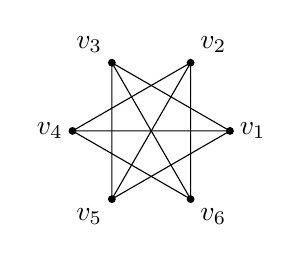
\begin{tikzpicture}
        \coordinate[label = right:$v_1$] (a) at (0:1);
        \coordinate[label = above right:$v_2$] (b) at (60:1);
        \coordinate[label = above left:$v_3$] (c) at (120:1);
        \coordinate[label = left:$v_4$] (d) at (180:1);
        \coordinate[label = below left:$v_5$] (e) at (240:1);
        \coordinate[label = below right:$v_6$] (f) at (300:1);
        
        \node at (a)[circle,fill,inner sep=1pt]{};
        \node at (b)[circle,fill,inner sep=1pt]{};
        \node at (c)[circle,fill,inner sep=1pt]{};
        \node at (d)[circle,fill,inner sep=1pt]{};
        \node at (e)[circle,fill,inner sep=1pt]{};
        \node at (f)[circle,fill,inner sep=1pt]{};

        \draw (a) -- (c) (a) -- (d) (a) -- (e);
        \draw (b) -- (d) (b) -- (e) (b) -- (f);
        \draw (c) -- (e) (c) -- (f);
        \draw (d) -- (f);
    \end{tikzpicture}
    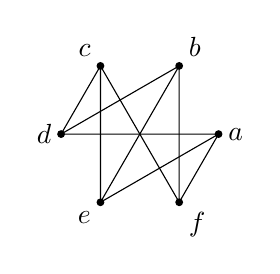
\begin{tikzpicture}
        \coordinate[label = right:$a$] (a) at (0:1);
        \coordinate[label = above right:$b$] (b) at (60:1);
        \coordinate[label = above left:$c$] (c) at (120:1);
        \coordinate[label = left:$d$] (d) at (180:1);
        \coordinate[label = below left:$e$] (e) at (240:1);
        \coordinate[label = below right:$f$] (f) at (300:1);
        
        \node at (a)[circle,fill,inner sep=1pt]{};
        \node at (b)[circle,fill,inner sep=1pt]{};
        \node at (c)[circle,fill,inner sep=1pt]{};
        \node at (d)[circle,fill,inner sep=1pt]{};
        \node at (e)[circle,fill,inner sep=1pt]{};
        \node at (f)[circle,fill,inner sep=1pt]{};

        \draw (a) -- (d) (a) -- (e) (a) -- (f);
        \draw (b) -- (d) (b) -- (e) (b) -- (f);
        \draw (c) -- (d) (c) -- (e) (c) -- (f);
    \end{tikzpicture}
    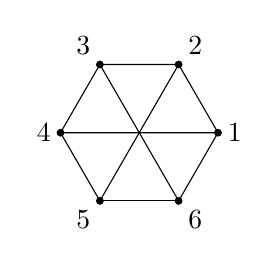
\begin{tikzpicture}
        \coordinate[label = right:$1$] (1) at (0:1);
        \coordinate[label = above right:$2$] (2) at (60:1);
        \coordinate[label = above left:$3$] (3) at (120:1);
        \coordinate[label = left:$4$] (4) at (180:1);
        \coordinate[label = below left:$5$] (5) at (240:1);
        \coordinate[label = below right:$6$] (6) at (300:1);
        
        \node at (1)[circle,fill,inner sep=1pt]{};
        \node at (2)[circle,fill,inner sep=1pt]{};
        \node at (3)[circle,fill,inner sep=1pt]{};
        \node at (4)[circle,fill,inner sep=1pt]{};
        \node at (5)[circle,fill,inner sep=1pt]{};
        \node at (6)[circle,fill,inner sep=1pt]{};

        \draw (1) -- (2) (1) -- (4) (1) -- (6);
        \draw (2) -- (3) (2) -- (5);
        \draw (3) -- (4) (3) -- (6);
        \draw (4) -- (5);
        \draw (5) -- (6);
    \end{tikzpicture}
\end{center}
    
    $G_1$ is not isomorphic to $G_2$ since $G_1$ contains a triangle and $G_2$ is bipartite. Recall that bipartite graphs contain no odd cycles. $G_2$ and $G_3$ are isomorphic. Take for example the function sending $a\rightarrow 1$, $b\rightarrow 3$, $c\rightarrow 5$, $d\rightarrow 2$, $e\rightarrow 4$, and $f\rightarrow 6$. Finally by transitivity of isomorphism $G_1$ and $G)_3$ are not isomorphic. 
    
    \question{Partial Fractions} Use partial fractions to determine and explicit formula for $[x^n]F(x)$ where $F(x)=\frac{1-6x+x^2}{(1-4x)(1-x)^2}$.
    \answer Observe the denominator is already factored so we have $\frac{1-6x+x^2}{(1-4x)(1-x)^2}=\frac{A}{(1-4x)}+\frac{Bx+C}{(1-x)^2}$. Solving for the constants we get $A=\frac{-7}{9}$, $B=\frac{-4}{9}$ and $C=\frac{16}{9}$. This gives $[x^n]F(x)=\frac{-7}{9}4^n+\frac{-4}{9}n(1)^{n}+\frac{16}{9}(1)^n=\frac{-7}{9}4^n+\frac{-4}{9}n+\frac{16}{9}$
    
    \newpage

    % oh no i was going to do this one - alena
    % ah sorry!!!! I misread and asked the wrong person
    % dw :) was just confused lol
    \question{Graph Construction} For $n \ge 2$, let $G_n$ be the graph whose vertices are permutations of $\{1, \dots, n\}$, where we have an edge between two permutations if we can obtain one from the other by swapping two elements. 
    \begin{enumerate}
        \item Draw $G_3$ and label its vertices. 
        \item Show that this graph is regular, find the degree.
        
    \end{enumerate}
    \answer \begin{enumerate}
        \item Using the notation $\sigma = (\sigma_1 , \sigma_2 , \sigma_3)$:

\begin{center}
    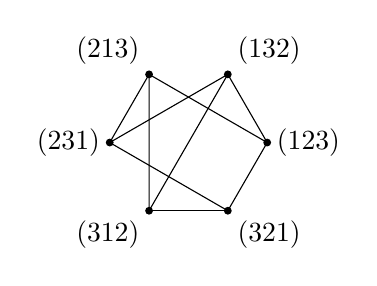
\begin{tikzpicture}
        \coordinate[label = right:$(123)$] (123) at (0:1);
        \coordinate[label = above right:$(132)$] (132) at (60:1);
        \coordinate[label = above left:$(213)$] (213) at (120:1);
        \coordinate[label = left:$(231)$] (231) at (180:1);
        \coordinate[label = below left:$(312)$] (312) at (240:1);
        \coordinate[label = below right:$(321)$] (321) at (300:1);
        
        \node at (123)[circle,fill,inner sep=1pt]{};
        \node at (132)[circle,fill,inner sep=1pt]{};
        \node at (213)[circle,fill,inner sep=1pt]{};
        \node at (231)[circle,fill,inner sep=1pt]{};
        \node at (312)[circle,fill,inner sep=1pt]{};
        \node at (321)[circle,fill,inner sep=1pt]{};

        \draw (123) -- (132) (123) -- (213) (123) -- (321);
        \draw (132) -- (231) (132) -- (312);
        \draw (213) -- (231) (213) -- (312);
        \draw (231) -- (321);
        \draw (312) -- (321);
    \end{tikzpicture}
\end{center}


        \item Degree should be $n \choose 2$ because a vertex $v$ will be adjacent to permutations that are obtained from $v$ by two elements swapping places, so we pick $2$ elements to swap out of $n$.
        
    \end{enumerate}
   
    \newpage
    
    \question{Compositions} How many integer compositions of $n$ consist of either 5 or 6 parts, where each part is even?
    \answer For a partition with only even parts, we want $A = \{2, 4, 6, \dots\}$ with weight function $w(a) = a$, which gives us generating series $\Phi_A(x) = x^2 + x^4 + x^6 + \dots = \frac{x^2}{1-x^2}$.
    
    The set we are counting is $A^5 \cup A^6$, which is a disjoint union, so we can apply the sum lemma to get $\Phi_S(x) = \Phi_{A^5}(x) + \Phi_{A^6}(x)$.

    By the product lemma, we have 
    \begin{center}
        $\Phi_{A^5}(x) = (\Phi_{A}(x))^5 = (\frac{x^2}{1-x^2})^5 =  \frac{x^{10}}{(1-x^2)^5}$

        $\Phi_{A^6}(x) = (\Phi_{A}(x))^6 = (\frac{x^2}{1-x^2})^6 =  \frac{x^{12}}{(1-x^2)^6}$
    \end{center}

    So \begin{center}
        $\Phi_S(x) = \frac{x^{10}}{(1-x^2)^5} + \frac{x^{12}}{(1-x^2)^6} = \frac{x^{10} - x^{12} + x^{12}}{(1-x^2)^6} = \frac{x^{10}}{(1-x^2)^6}$
    \end{center}

    The number of integer compositions of $n$ consisting of 5 or 6 even parts is 

    \begin{center}
        $[x^n]\Phi_S(x) = [x^n]\frac{x^{10}}{(1-x^2)^6} = [x^{n-10}](1-x^2)^{-6} =  \begin{cases} 
          0 & n\ \mathrm{is}\ \mathrm{odd} \\
          {\frac{n-10}{2} + 5 \choose 5} & n\ \mathrm{is}\ \mathrm{even} 
       \end{cases}$
    \end{center}

    
    
\end{enumerate}



%\title{Math 239 Fall 2023 Tutorial Questions Week 8}

\date{2023 Nov. 9/10}
\maketitle

\begin{enumerate}

    \question{Exotic Cubes} Let $C_{n,m}$ be the graph where the vertices are the elements of $\{ 0, 1 , \cdots, m-1\}^n$, and where there is an edge between $v_1$ and $v_2$ iff $v_1 $ and $v_2$ differ by exactly $1$ in exactly one coordinate. For example if $n=2$ and $m=3$ the vertex $(1,2)$ to the vertices $(0,2) , (2,2) , (1,1)$.
    \begin{enumerate}
        \item Draw $C_{2,3}$.
        \item Is $C_{n,m}$ bipartite?
        \item What is the maximum degree of a vertex in $C_{n,m}$? What about the minimum?
        \item (hard, attempt other questions first) What is the number of edges in $C_{n,m}$?
    \end{enumerate}
    
    % We write $K_{n_1 , \cdots, n_k}$ to be the graph with $|V_j| = n_j$, and $uv \in E$ iff $u \in V_a, v \in V_b$ where $a \neq b$ (ie if two vertices are in different parts there is an edge between them). Note that $K_{n_1 , \cdots, n_k}$ has $n_1 + \cdots + n_k$ vertices. This is called the \textbf{complete $k$-partite graph on $n_1 , \cdots, n_k$ vertices}.

    
    
    
    \question{Find the Mistake} The following is a false statement and a false proof. Identify the error in the provided proof and consider how to avoid making this mistake in general. Can you think of a way to make the theorem true? If so, prove it. 
    \\
    \textbf{Non-theorem:} If $G$ is a graph with $|V(G)|\geq 4$ and minimum degree at least $2$, then $G$ contains a cycle of length at least $4$.
    \\
    \textbf{Non-proof:} We proceed by induction on $|V(G)|$. We begin with the base case: Let $G$ be a graph with four vertices and minimum degree at least $2$. Suppose for a contradiction that $G$ does not contain a cycle of length $4$. Since $G$ has minimum degree at least two, it follows that $G$ contains a cycle: and since $G$ does not contain a cycle of length $4$, it therefore contains a cycle of length $3$. Let $v$ be the vertex not in this cycle of length three. Since $G$ has minimum degree at least $2$ and $|V(G)|=4$, it follows that $v$ is adjacent to at least two vertices in this cycle. Then $G$ does contain a cycle of length $4$, a contradiction. Thus the base case holds. To prove the inductive step, let $H$ be a graph on $n-1$ vertices for which the theorem holds. Construct a new graph $G$ on $n$ vertices by adding a new vertex to $H$ with at least two incident edges. Since $H$ contains a cycle of length $4$ by induction, $G$ contains a cycle of length $4$ and the result holds. 
    
    
    \question{Pr{\"u}fer Codes} Let $n \ge 3$, and suppose we have a tree on vertex set $\{1, \dots, n\}$. We can construct a sequence of elements from $\{1, \dots, n\}$ algorithmically as follows:
    \begin{enumerate}[label=\arabic*)]
        \item Check to make sure the tree has more than a single edge. If not, terminate.
        \item Find the leaf with the smallest label. Add the label of its neighbor to the sequence. Delete the leaf from the graph and repeat.
    \end{enumerate}
    Notice that this will produce a sequence of length $n - 2$, as we're terminating the algorithm when we have a single edge (two vertices) left. The sequence we get from this algorithm is called a Pr{\"u}fer sequence.

    \begin{enumerate}
        \item Write the Pr{\"u}fer sequences for the following trees:

        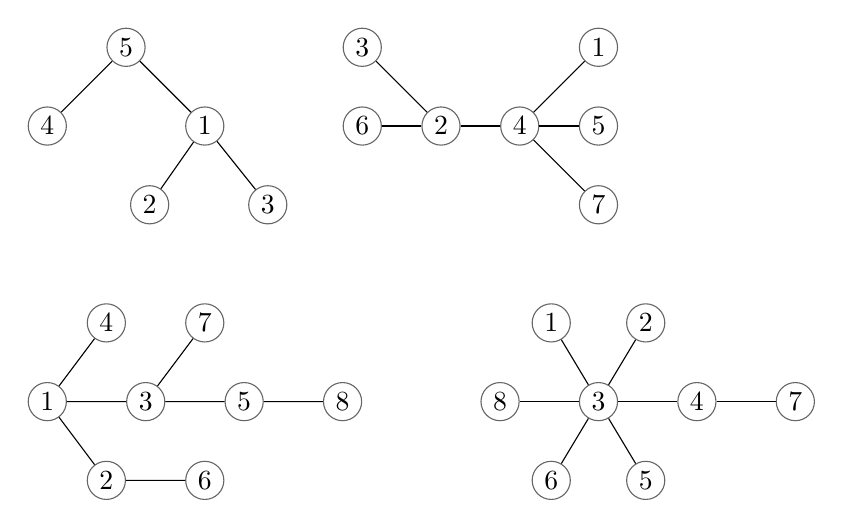
\begin{tikzpicture}[shorten >=1pt,->]
  \tikzstyle{vertex}=[circle,draw=black!60,minimum size=12pt,inner sep=2pt]
  \node[vertex] (G_4) at (-1,-1) {4};
  \node[vertex] (G_5) at (0,0)   {5};
  \node[vertex] (G_1) at (1,-1)  {1};
  \node[vertex] (G_2) at (0.3,-2)  {2};
  \node[vertex] (G_3) at (1.8,-2)  {3};
  \draw (G_4) -- (G_5) -- (G_1) -- (G_2) -- cycle;
  \draw (G_1) -- (G_3) -- cycle;

\node[vertex] (G_6') at (3,-1) {6};
\node[vertex] (G_3') at (3,0) {3};
  \node[vertex] (G_2') at (4,-1)   {2};
  \node[vertex] (G_4') at (5,-1)  {4};
  \node[vertex] (G_1') at (6,0)  {1};
  \node[vertex] (G_5') at (6,-1)  {5};
  \node[vertex] (G_7') at (6,-2)  {7};
  \draw (G_6') -- (G_2') -- (G_4') -- (G_5') -- cycle;
  \draw (G_4') -- (G_1') -- cycle;
  \draw (G_3') -- (G_2') -- cycle;
  \draw (G_4') -- (G_7') -- cycle;

  \node[vertex] (G_4'') at (-0.25,-3.5) {4};
  \node[vertex] (G_1'') at (-1,-4.5)   {1};
  \node[vertex] (G_2'') at (-0.25,-5.5)  {2};
  \node[vertex] (G_6'') at (1,-5.5)  {6};
  \node[vertex] (G_3'') at (0.25,-4.5)  {3};
  \node[vertex] (G_7'') at (1,-3.5)  {7};
  \node[vertex] (G_5'') at (1.5,-4.5)  {5};
  \node[vertex] (G_8'') at (2.75,-4.5)  {8};
  \draw (G_1'') -- (G_4'') -- cycle;
  \draw (G_6'') -- (G_2'') -- (G_1'') -- (G_3'') -- (G_5'') -- (G_8'') -- cycle;
  \draw (G_3'') -- (G_7'') -- cycle;

  \node[vertex] (H_3) at (6,-4.5) {3};
  \node[vertex] (H_1) at (5.4,-3.5)   {1};
  \node[vertex] (H_2) at (6.6,-3.5)   {2};
  \node[vertex] (H_4) at (7.25,-4.5)  {4};
  \node[vertex] (H_7) at (8.5,-4.5)  {7};
  \node[vertex] (H_8) at (4.75,-4.5)  {8};
  \node[vertex] (H_6) at (5.4,-5.5)   {6};
  \node[vertex] (H_5) at (6.6,-5.5)   {5};
  
  \draw (H_8) -- (H_3)  -- (H_4)  -- (H_7) -- cycle;
  \draw (H_1) -- (H_3)  -- (H_5)  -- cycle;
  \draw (H_2) -- (H_3)  -- (H_6)  -- cycle;
    
\end{tikzpicture}

\hfill
                
        \item Can any sequence of $n-2$ numbers from $\{1, \dots, n\}$ be the Pr{\"u}fer sequence of a tree on $n$ vertices? Construct an algorithm for building a labeled tree out of a given sequence, or explain why it's not possible. 

        \item Use Pr{\"u}fer sequences to count the number of labelled trees on $n$ vertices. (Hint: The algorithm you wrote in part (b) gives you a mapping that is the inverse of the mapping from labeled trees to their Pr{\"u}fer sequences. You do not need to prove that it's a bijection.)

        \item (hard, attempt other questions first) Prove that the algorithm gives us a bijective mapping. 
    \end{enumerate}
    
    
    \question{Spanning Tree} Let $e$ be an edge in a connected graph $G$. Prove that $e$ is a bridge in $G$ if and only if $e$ is in every spanning tree of $G$.

    \question{Bonus: Complete $k$-partite Graphs} We say a graph $G=(V,E)$ is \textbf{$k$-partite} if we can partition $V = V_1 \sqcup \cdots \sqcup V_k$ ($\sqcup$ indicates \textit{disjoint} union, and the $V_j$ are called \textit{parts}) such that there are no edges between distinct elements of $V_j$ (where $j = 1, \cdots, k$). Find a tight bound on the number of edges in a $k$-partite graph with $kn$ vertices, and say when this tight bound occurs.
\end{enumerate}
 % \title{Math 239 Fall 2023 Tutorial Questions Week 9}

\date{2023 Nov. 16/17}
\maketitle

\begin{enumerate}
    \question{Planar or Not}For each of the following graphs, find a planar embedding or an edge subdivision of $K_5$ or $K_{3,3}$. In the latter case, mark the edges in the subdivision of $K_5$ or $K_{3,3}$. 
    \begin{figure}[h]
        \centering
        \includegraphics[width=.45\textwidth]{planar.png}\hfill
        \includegraphics[width=.45\textwidth]{nonplanar.png}
    \end{figure}
    
    \question{Euler's Formula} Suppose $G$ is a connected planar embedding where every vertex has degree $2$ or $5$ and every face has degree $4$.
    \begin{enumerate}
        \item Determine a formula for the number of edges in terms of the number of vertices of degree 5.
        \item Suppose there are exactly $4$ vertices of degree $5$. Determine the number of edges, faces, and vertices of degree $2$. Draw a planar embedding that satisfies these parameters.
    \end{enumerate}

    
    \question{Complete Planar Tripartite Graphs} For positive integers $a \geq b \geq c$ define $K_{a,b,c}$ to be the \textbf{complete tripartite graph} with a tripartition $A,B,C$ (with $|A| = a$ etc.) such that $uv \in E$ iff $u$ and $v$ are in different parts. What are the possible values of $(a,b,c)$ such that $K_{a,b,c}$ is planar? Ignore the trivial cases where any of $a,b,c$ are $0$.

    
    \question{Partitioning Into Planar} Let $n \ge 6$. Prove that the it is not possible to partition the edges of $K_n$ into $\lfloor \frac{n}{6} \rfloor$ planar subgraphs.

    \question{Bonus Question: The Pentagon Problem}
    Let $G$ be a $5$-cycle (a pentagon) with vertices enumerated $1 ,2,3,4,5$ in a circle. Let $c = (c_1 , c_2, c_3, c_4, c_5)$ denote certain numbers we put on vertex $1,2,3,4,5$ respectively (so vertex $3$ has the value $c_3$ on it). We let $c_j \in \mathbb{Z}$, but we requires that $c_1 + c_2 + c_3 + c_4 + c_5 \geq 1$. Now play the following game:
    \begin{itemize}
        \item[] If we have all $c_j>0$ then we have won. Otherwise pick a vertex $j$ with $c_j < 0$. Then ``activate" the vertex to get a new configuration $c'$ with
        \begin{align*}
            c'_i = \begin{cases}
                c_i & \text{if $i$ is not adjacent to $j$},\\
                c_{i} + c_j & \text{if $i$ is adjacent to $j$},\\
                c_{i} - 2c_i & \text{if $i = j$}.
            \end{cases}
        \end{align*}
        Then continue the game from the start with the configuration $c'$.
    \end{itemize}
    Show that we always win, so we always reach a state where $c_j > 0$ for all initial $c$'s.

    This problem is sourced from \textit{The Mathematics of Chip-Firing} by Klivans (problem $2.8.17$). I have no idea how to do it.
\end{enumerate}
% \title{Math 239 Fall 2023 Tutorial Questions Week 10}

\date{2023 Nov. 23/24}
\maketitle

\begin{enumerate}
    \question{Planarity and Graph Complements} 
    \begin{enumerate}
        \item  For each $k\in\{ 5,6\}$ give two non-isomorphic graphs $G_1$ and $G_2$ with $k$ vertices each such that $G_1, G_2, \overline{G_1}, \overline{G_2}$ are planar. Prove they are planar(give a planar embedding) and give a one sentence proof that $G_1$ and $G_2$ are non-isomorphic. 
        \item Describe a graph $G$ where $\overline{G}$ and $G$ are both non-planar. 
     \end{enumerate}
    
    \question{Cartesian Product of Graphs} The \textit{Cartesian Product} of two graphs $G$ and $H$, denoted $G\square H$ is defined as 
    \[V(G\square H) = V(G) \times V(H)\]
    and if two vertices $(a_1, b_1)$ and $(a_2, b_2)$ are adjacent in $G \square H$ if and only if either 
    \begin{itemize}
        \item $a_1 = a_2$ and $b_1$ is adjacent to $b_2$ in H, or
        \item $b_1 = b_2$ and $a_1$ is adjacent to $a_2$ in G, 
    \end{itemize}
i.e.
    \[E(G\square H) = \{(a_1,b_1)(a_2,b_2): a_1 = a_2 \text{ and } b_1b_2\in E(H)\text{, or, }a_1a_2 \in E(G) \text{ and } b_1 = b_2\}\]
    \begin{enumerate}
        \item Suppose that $\phi_1$ is a $k$-coloring of $G$ (assigning colors $\{1,\cdots,k\}$ ) and  $\phi_2$ is a $k$-coloring of $H$ (assigning colors $\{1,\cdots,k\}$ ) for some positive integer $k$. Define\[\phi((a,b)) := \phi_1(a) + \phi_2(b)\mod{k}.\]
        Prove that $\phi$ is a $k$-coloring of $G\square H$.
        \item Deduce that if $G$ is $k_1$-colorable and $H$ is $k_2$-colorable, then $G\square H$ is $\max \{k_1, k_2\}$-colorable.
    \end{enumerate}

    
    \question{Graph Coloring} Let $k \ge 1$. Let $G$ be a graph where every nonempty subgraph has a vertex of degree at most $k$. Prove that $G$ is $(k + 1)$-colourable. Find an example of $G$ where $G$ is not $k$-colourable.

    
    \question{A Second Planarity Question} Determine whether or not each of the following graphs is planar. If so, give a planar embed- ding. If not, exhibit an edge subdivision of $K_5$ or $K_{3,3}$ in the graph.
    \begin{center}
    \includegraphics[scale=0.4]{t10q4drawings.png}
    \end{center}
    
    % \newpage
    
    \question{Bonus Question: Spectral Graph Theory}
    The Laplacian operator on $\mathbb{R}^n$, which acts on functions $\mathbb{R}^n \to \mathbb{R}$ by sending $f$ to $\Delta f = \sum_{i = 1}^n \frac{\partial^2 f}{\partial x_i^2}$. The Laplacian operator notionally measures how much $f$ at $p$ differs from points near $p$. It turns out this plays a large role in a theory of mathematics called spectral theory, which is concerned with finding functions $f$ such that $\Delta f = \lambda f$ (so-called ``eigenfunctions").

    There is a graph theory equivalent of the Laplacian. Let $G$ be a graph with $n$ vertices, labelled $1 , \cdots , n$. Then Define the \textbf{degree matrix} $D_G$ of $G$ as the $n \times n$ matrix
    \begin{align*}
        D_G(i,j) = \begin{cases}
            \deg (v_i) & \text{ if } i=j,\\
            0 & \text{ else}.
        \end{cases}
    \end{align*}
    Define as well the \textbf{adjacency matrix} $A_G$ of $G$ as the (symmetric) $n \times n$ matrix
    \begin{align*}
        A_G(i,j) = \begin{cases}
            -1 & \text{ if } v_i v_j \in E,\\
            0 & \text{ else}.
        \end{cases}
    \end{align*}
    Now finally define the \textbf{graph Laplacian} of $G$ as $L = L_G = D_G - A_G$. Since this is an $n \times n$ real symmetric matrix, there are $n$ real eigenvalues (counted with multiplicity). This is exactly the provenance of \textbf{spectral graph theory}. We call the multiset of eigenvalues the \textbf{spectrum} of a graph, and often write them in increasing order $\lambda_1 \leq \cdots \leq \lambda_n$ (so that $\lambda_1$ is the lowest eigenvalue of $G$).
    \begin{enumerate}
        \item Argue that for any $G$ then $L (1, \cdots, 1)^T = 0$, and so $0$ is always an eigenvalue of $G$.
        \item Find the spectrum of $K_n$, $K_{n,n}$, $P_n$, $C_n$, the star graph $S_n$, and the $n$-cube $Q_n$.
        \item Prove that if $G$ is connected then $\lambda_1> 0$.  Further show that if $\lambda_i = 0$ and $\lambda_{i+1} \neq 0$ then $G$ has exactly $i+1$ connected components.
    \end{enumerate}
\end{enumerate}
\title{Math 239 Fall 2023 Tutorial Review Session}

\date{2023 Nov. 30/Dec. 1}
\maketitle

\begin{enumerate}
    \question{Compositions} Find the generating function for number of compositions with at least $3$ parts where each part is an even number greater than $3$.
    \answer Each part has generating function
    \begin{align*}
        P(x) = x^4 + x^6 + x^8 + \cdots = \frac{x^4}{1-x^2}.
    \end{align*}
    Then the GF for the whole thing is
    \begin{align*}
        C(x) = P(x)^3 + P(x)^4 + P(x)^5 + \cdots = \frac{P(x)^3}{1-P(x)} = \frac{x^{12}}{1-3x^2 +2x^4 +x^6 -x^8}.
    \end{align*}
    
    \question{Sequences} Give the generating functions of the following sequences. Give a recursion that these sequences satisfy.
    \begin{enumerate}
        \item $a_n = 3 + 3(2^n)$.
        \item $b_n = \lfloor \frac{n}{2} \rfloor$ (so $0,0,1,1,2,2, \cdots$).
        % \item $c_n = \frac{1}{n}$ for $n >1$, $c_0 = 0$.
    \end{enumerate}
    \answer 
    \begin{enumerate}
        \item $A(x) = 3 \sum x^n + 3 \sum(2x)^n = \frac{3}{1-x} + \frac{3}{1-2x} = \frac{6 - 9 x}{2 x^2 - 3 x + 1}$.
        Then the recursion with characteristic polynomial $2 x^2 - 3 x + 1$ is
        \begin{align*}
            a_n = 3a_{n-1} - 2a_{n-2}, \qquad a_{0} = 6 , a_{1} = 9.
        \end{align*}
        \item First recall/note that $\sum_{n \geq 0} n x^n = \frac{x}{(1-x)^2}$.
        \begin{align*}
            B(x) &= 0x^0 + 0x + 1x^2 + 1x^3 + 2x^4 + 2x^5 + \cdots\\
            &= \left( 0x^0 + 1x^2 + 2x^4 + \cdots \right) + x\left( 0x^0 + 1x^2 + 2x^4 + \cdots\right)\\
            &= \sum_{n \geq 0} \left(  n x^{2n} \right) + x \sum_{n \geq 0} \left(  n x^{2n} \right)\\
            &= \frac{x^2}{(1-x^2)^2} + \frac{x^3}{(1-x^2)^2}\\
            &= \frac{x^2}{x^3 - x^2 - x + 1}
        \end{align*}
        This gives a recursion of
        \begin{align*}
            a_n = a_{n-1} + a_{n-2} - a_{n-3}, \qquad a_0 = 0, a_1 = 0, a_2 = 1.
        \end{align*}
    \end{enumerate}
    
    \question{Trees} Let $T$ be a tree with $|V(T)|\geq 2$ and no vertices of degree two. Prove that more than half of the vertices of $T$ are leaves.
    \answer Let $n=|V(T)|$. Since $T$ is a tree $|E(T)|=n-1$. By the handshaking lemma, 
    \begin{align*}
        \sum_{v\in V(T)} deg(v)=2|E(T)|=2(n-1).    
    \end{align*} 
    Let $L$ be the set of leaves in $T$ and $|L|=l$. Since $T$ has no vertices of degree two 
    \begin{align*}
            l+\sum_{v\notin L} deg(v)=2n-2\geq l+3(n-l)=3n-2l.    
    \end{align*}
    Hence $2l\geq n+2$ and thus $l\geq \frac{n}{2}+1$ and the result follows. 
    
    \question{Cycles} Let $G$ be a connected graph on $n\geq 1$ vertices with $n$ edges.
    \begin{enumerate}
        \item Prove that the average degree of the vertices of $G$ is 2.
        \item Prove that $G$ has a unique cycle.
    \end{enumerate}
    \answer 
    \begin{enumerate}
        \item By the handshaking lemma, $\sum_{v\in V(G)} deg(v)=2|E(G)|=2n=2|V(G)|$. Thus $\frac{1}{|V(G)|}\sum_{v\in V(G)}deg(v)=2$. 
        \item Since $n>n-1$, $G$ is not a tree. Thus $G$ contains a cycle. For the sake of contradiction suppose $G$ contains two distinct cycles $C_1$ and $C_2$. Since the cycles are distinct $C_1$ contains some edge $e_1$ such that $e_1$ is not in $C_2$ and $C_2$ contains some edge $e_2$ such that $e_2$ is not in $C_1$. Since $e_1$ and $e_2$ are in cycles, $e_1$ and $e_2$ are not bridges in $G$. Since $e_1$ is not a bridge $G-e_1$ is still connected. Since $e_1$ is not in $C_2$, $C_2$ is still a cycle in $G-e_1$, so $e_2$ is still not a bridge. Thus $G'=G-e_1-e_2$ is connected. However $|E(G')|=n-2$ which contradicts $G'$ being connected since the minimum number of edges a connected graph on $n$ vertices can have is $n-1$. Thus $G$ contains exactly one cycle. 
    \end{enumerate}
    
    \question{Planar Embedding} Let $G$ be a connected planar graph. Prove that if $G$ is not bipartite, then any planar embedding of $G$ has at least 2 faces with odd degree.
    \answer Since $G$ is not bipartite, $G$ contains an odd cycle $C$. Let $F_1, \dots, F_k$ be the faces inside $C$ in the planar embedding. Consider the sum of the degrees of the faces. 
    \begin{itemize}
        \item Each edge in $C$ gets counted once
        \item Let $D$ be the set of edges on any boundary of any $F_i$, but not on $C$. 
    \end{itemize}
    Each edge in $D$ is counted twice. So $\sum_i \mathrm{deg}(F_i) = |E(C)| + 2|D|$. Since $|E(C)|$ is odd and $2|D|$ is even, $\sum_i \mathrm{deg}(F_i)$ is odd, so $deg(F_i)$ must be odd for some $i$, and therefore we have at least one face inside $C$ with odd degree. We can use a similar argument for the existence of a face outside $C$ with odd degree, so there must be at least two faces with odd degree. 
    
    % \question{Bridges} Let $G$ be a 4-regular graph. Prove that $G$ does not have a bridge. (Note: $G$ is not necessarily connected.)
    % \answer Suppose for contradiction that $e = uv$ is a bridge in $G$, and let $H$ be the component of $G$ that contains $e$. Then $H - e$ has two components, which we will call $H_1$ and $H_2$. Suppose $u \in V(H_1)$. Since $G$ is 4-regular, every vertex in $H_1$ has degree 4, except $u$ (since we removed edge $e=uv$). Then $H_1$ is a graph with an odd number (one) of vertices with odd degree (3), which is a contradiction. Therefore, no bridge can exist.

    \question{Matching} Let $G$ be a graph on $n$ vertices where $n$ is even. Suppose that $deg_G(v) \geq n/2$ for all $v \in V(G).$ Prove that $G$ has a perfect matching.

   Hint: Prove that if $M$ is a matching that is not perfect, then there exists an augmenting path with respect to $M$ of length $1$ or $3$.
    \answer 
    Suppose not (for a contradiction). Let $M$ be a maximum matching of $G$. Let $e_1 = u_1v_1, e_2 = u_2v_2, \cdots, e_k=v_ku_k$ be the edges of $M$. Let $X = \{u_i, v_i: i \in \{1, \cdots, k\}\}$. Note that $|X| = 2k$.
    
    First suppose there exists an edge $e=uv \in E(G)$ where $u, v \not \in X$. But then $e$ is an $M$-augmenting path of length one, contradicting Lemma 8.1.1 as $M$ is maximum.

    So we assume that for every edge $e = uv \in E(G)$, we have $\{u,v\} \cap X \neq \empty$ (that is, $X$ is a cover of $G$). Since $M$ is not perfect, we have that $k < n/2$ and hence $|X| < n$. Since $|X|$ is even and $n$ is even, it follows that $|X| \leq n-2$. Thus there exists distinct $u,v\in V(G) \setminus X$.

    Since $X$ is a cover of $G$, we find that $N_G(u) \subseteq X$ and similarly $N_G(v) \subseteq X$.

    First suppose there exists $i \in \{1, \cdots, k\}$ such that $|N_G(u) \cap \{u_i, v_i\}| + |N_G(v) \cap \{u_i, v_i\}| \geq 3$.

    Without loss of generality, we assume that $u_i, v_i \in N_G(u)$; similarly without loss of generality, we assume that $v_i \in N_G(v)$. But then $P = uu_iv_iv$ is an $M$-augmenting path of $G$, contradicting Lemma 8.1.1 as $M$ is maximum.

    So we assume that for every $i \in \{1, \cdots, k\}$ we have that
    \[|N_G(u) \cap \{u_i, v_i\}| + |N_G(v) \cap \{u_i, v_i\}| \leq 2.\]
    But then summing over $i$ and using that $N_G(u), N_G(v) \subseteq X$, we find that 
    \[|N_G(u)| + |N_G(v)| \leq \sum_{i=1}^k |N_G(u) \cap \{u_i, v_i\}| + |N_G(v) \cap \{u_i, v_i\}| \leq 2k < n.\]
    
    Yet by assumption every vertex of $G$ has degree at least $n/2$ and hence 
    \[|N_G(u)| + |N_G(v)| = deg_G(u) + deg_G(v) \geq n/2 + n/2 = n,\]
    contradicting the previous inequality.

    \question{Cover} Let $G$ be a bipartite graph with bipartition $(A,B)$, and let $C_1$ and $C_2$ be covers of $G$. Define 
    \[C_3 := \left( (C_1 \cap C_2) \cap A \right) \cup ((C_1 \cup  C_2) \cap B)\]
    \begin{enumerate}
        \item Show that $C_3$ is a cover.
        \item Show that if $C_1$ and $C_2$ are minimum covers of $G$, then $C_3$ is a minimum cover of $G$.
    \end{enumerate}
    \answer 
    \begin{enumerate}
        \item By definition of cover, it suffices to show that for each $ab \in E(G)$, we have $a \in C_3$ or $b \in C_3$. Without loss of generality, we assume that $a \in A$ and $b \in B$.

        Since $C_1$ is a cover, we have by definition of cover that $a \in C_1$ or $b\in C_1$. Similarly since $C_2$ is a cover, we have $a\in C_2$ or $b\in C_2$.

        First suppose that $b\in C_1$. Then $b\in C_1 \cup C_2$. Since $b \in B$, we have $b \in (C_1 \cup C_2) \cap B \subseteq C_3$ as desired.

        So we assume $b \not \in C_1$ and hence $a \in C_1$. 
        Similarly if $b \in C_2$, then $b \in C_3$ as desired. So we assume $b \not \in C_2$ and hence $a \in C_2$.

        But then $a \in C_1 \cap C_2$. Since $a \in A,$ we have $a \in (C_1 \cap C_2) \cap A \subseteq C_3$ and hence $a \in C_3$ as desired.
        \item Since $C_1$ and $C_2$ are minimum covers of $G$, we have that $|C_1| = |C_2|.$ By (a), $C_3$ is a cover. Let 
        \[C_4 := ((C_1 \cap C_2)\cap B) \cup ((C_1 \cup C_2) \cap A).\]
        By applying (a) symmetrically to the bipartition $(B,A)$ we find that $C_4$ is also a cover of $G$.
        Since $C_1$ and $C_2$ are minimum covers of $G$, we have that $|C_1| \leq |C_3|$ and $|C_2| \leq C_4$. Hence
        \begin{align*}
            |C_1| + |C_2| \leq |C_3| + |C_4| &= |(C_1 \cap C_2) \cap A| +|(C_1 \cup C_2) \cap B|\\ & + |(C_1 \cup C_2) \cap A|  + |(C_1 \cap C_2) \cap B| \\
            &= |C_1 \cap A| + |C_2 \cap A| + |C_1 \cap B| + |C_2 \cap B| \\
            &= |C_1| + |C_2|.
        \end{align*}
        Thus equality holds through out and we find that $|C_3| + |C_4| = |C_1| + |C_2|.$ Since $|C_1| \leq |C_3|$ and $|C_2| \leq |C_4|$, it follows that $|C_3|=|C_4| = |C_1| = |C_2|$. That is, $C_3$ and $C_4$ are also minimum covers of $G$ as desired.
    \end{enumerate}
\end{enumerate}
% \title{Math 239 Fall 2023 Tutorial Questions Week 12}

\date{2023 Dec. 7/8}
\maketitle

\begin{enumerate}
    \question{Title for Question 1} blah blah.

    
    \question{Title for Question 2} blah blah.

    
    \question{Title for Question 3} blah blah.

    
    \question{Title for Question 4} blah blah.
\end{enumerate}
% \title{Math 239 Fall 2023 Tutorial Questions Week 13}

\date{2023 Dec. 14/15}
\maketitle

\begin{enumerate}
    \question{Title for Question 1} blah blah.

    
    \question{Title for Question 2} blah blah.

    
    \question{Title for Question 3} blah blah.

    
    \question{Title for Question 4} blah blah.
\end{enumerate}

\end{document}
